% answers.tex —— 2015 年·广东卷·理科 · 参考答案与详细解析片段
% 由 tools/generate_projects.py 依来源总账自 2015/2015_数学真题_广东理_试题.md + 2015/2015_数学真题_广东理_解析正文.md + 2015/2015_数学真题_广东理_答案要点.md 生成，勿手改（改源 MD 后重跑）

\begin{gktip}
固定原卷不附参考答案（证据等级 D）；以下推导由项目独立完成，并经独立角色盲核，不作为官方解析。
\end{gktip}

\begin{answer}
\gksolhead{1}{集合运算}

\textbf{题目}：

若集合 \(M=\{x\mid (x+4)(x+1)=0\}\)，\(N=\{x\mid (x-4)(x-1)=0\}\)，则 \(M\cap N=\)（　）

(A) \(\{1,4\}\)　(B) \(\{-1,-4\}\)　(C) \(\{0\}\)　(D) \(\varnothing\)

\Needspace{4\baselineskip}
\textbf{解析}

\Needspace{5\baselineskip}
解方程得
\nopagebreak[4]
\[
M=\{x\mid (x+4)(x+1)=0\}=\{-4,-1\},\qquad
N=\{x\mid (x-4)(x-1)=0\}=\{4,1\}.
\]
\Needspace{5\baselineskip}
\(M\) 的元素全为负整数，\(N\) 的元素全为正整数，两者无公共元素，故
\nopagebreak[4]
\[
M\cap N=\varnothing.
\]

故选 (D)。

（验证：逐一比对 \(-4,-1\notin N\)，\(4,1\notin M\)；两集合元素个数之和为 \(4\)，与 \(M\cup N=\{-4,-1,1,4\}\) 的四个元素一致。）

\gkanswer{答案：D}

\end{answer}
\begin{answer}
\gksolhead{2}{复数}

\textbf{题目}：

若复数 \(z=\mathrm{i}(3-2\mathrm{i})\)（\(\mathrm{i}\) 是虚数单位），则 \(\overline{z}=\)（　）

(A) \(2-3\mathrm{i}\)　(B) \(2+3\mathrm{i}\)　(C) \(3+2\mathrm{i}\)　(D) \(3-2\mathrm{i}\)

\Needspace{4\baselineskip}
\textbf{解析}

\Needspace{5\baselineskip}
由 \(\mathrm{i}^2=-1\)，
\nopagebreak[4]
\[
z=\mathrm{i}(3-2\mathrm{i})=3\mathrm{i}-2\mathrm{i}^2=2+3\mathrm{i}.
\]
\Needspace{5\baselineskip}
共轭复数实部相同、虚部取相反数，故
\nopagebreak[4]
\[
\overline{z}=2-3\mathrm{i}.
\]

故选 (A)。

（验证：\(\operatorname{Re}z=2\)，\(\operatorname{Im}z=3\)，取共轭后实部不变、虚部变号；与 (A) 逐项一致。）

\gkanswer{答案：A}

\end{answer}
\begin{answer}
\gksolhead{3}{函数奇偶性}

\textbf{题目}：

下列函数中，既不是奇函数，也不是偶函数的是（　）

(A) \(y=\sqrt{1+x^2}\)　(B) \(y=x+\dfrac{1}{x}\)　(C) \(y=2^x+\dfrac{1}{2^x}\)　(D) \(y=x+\mathrm{e}^x\)

\Needspace{4\baselineskip}
\textbf{解析}

四个函数的定义域均关于原点对称。记所给函数为 \(f(x)\)，分别计算 \(f(-x)\)：

(A) \(f(-x)=\sqrt{1+(-x)^2}=\sqrt{1+x^2}=f(x)\)，为偶函数。

(B) \(f(-x)=-x+\dfrac{1}{-x}=-x-\dfrac{1}{x}=-f(x)\)，为奇函数。

(C) \(f(-x)=2^{-x}+\dfrac{1}{2^{-x}}=2^{-x}+2^{x}=f(x)\)，为偶函数。

(D) \(f(-x)=-x+\mathrm{e}^{-x}\)。取 \(x=1\)：\(f(1)=1+\mathrm{e}\)，\(f(-1)=-1+\mathrm{e}^{-1}\)，二者既不相等也不互为相反数（\(f(-1)\approx-0.632\)，\(f(1)\approx3.718\)，\(-f(1)\approx-3.718\)），故 (D) 既不是奇函数也不是偶函数。

故选 (D)。

（验证：前三个选项已由定义直接判定；(D) 用 \(x=1\) 与 \(x=-1\) 两点排除奇偶性，不必讨论恒等式。）

\gkanswer{答案：D}

\end{answer}
\begin{answer}
\gksolhead{4}{古典概型}

\textbf{题目}：

袋中共有 15 个除了颜色外完全相同的球，其中有 10 个白球，5 个红球。从袋中任取 2 个球，所取的 2 个球中恰有 1 个白球，1 个红球的概率为（　）

(A) \(\dfrac{5}{21}\)　(B) \(\dfrac{10}{21}\)　(C) \(\dfrac{11}{21}\)　(D) \(1\)

\Needspace{4\baselineskip}
\textbf{解析}

\Needspace{5\baselineskip}
从 \(15\) 个球中任取 \(2\) 个，基本事件总数为
\nopagebreak[4]
\[
\binom{15}{2}=\frac{15\cdot14}{2}=105.
\]
\Needspace{5\baselineskip}
恰有 \(1\) 个白球、\(1\) 个红球的取法数为
\nopagebreak[4]
\[
\binom{10}{1}\binom{5}{1}=10\cdot5=50.
\]
\Needspace{5\baselineskip}
故所求概率
\nopagebreak[4]
\[
P=\frac{50}{105}=\frac{10}{21}.
\]

故选 (B)。

（验证：用对立事件核对：同色取法为 \(\binom{10}{2}+\binom{5}{2}=45+10=55\)，同色概率 \(55/105=11/21\)，于是 \(1-11/21=10/21\)，与直接计算一致。）

\gkanswer{答案：B}

\end{answer}
\begin{answer}
\gksolhead{5}{直线与圆相切}

\textbf{题目}：

平行于直线 \(2x+y+1=0\) 且与圆 \(x^2+y^2=5\) 相切的直线的方程是（　）

(A) \(2x+y+5=0\) 或 \(2x+y-5=0\)

(B) \(2x+y+\sqrt{5}=0\) 或 \(2x+y-\sqrt{5}=0\)

(C) \(2x-y+5=0\) 或 \(2x-y-5=0\)

(D) \(2x-y+\sqrt{5}=0\) 或 \(2x-y-\sqrt{5}=0\)

\Needspace{4\baselineskip}
\textbf{解析}

\Needspace{5\baselineskip}
与直线 \(2x+y+1=0\) 平行的直线可设为
\nopagebreak[4]
\[
2x+y+c=0.
\]
\Needspace{5\baselineskip}
圆 \(x^2+y^2=5\) 的圆心为原点，半径 \(r=\sqrt{5}\)。直线与圆相切等价于圆心到直线的距离等于半径：
\nopagebreak[4]
\[
\frac{|c|}{\sqrt{2^2+1^2}}=\sqrt{5}
\ \Longrightarrow\ \frac{|c|}{\sqrt{5}}=\sqrt{5}
\ \Longrightarrow\ |c|=5.
\]
\Needspace{5\baselineskip}
故 \(c=\pm5\)，所求直线为
\nopagebreak[4]
\[
2x+y+5=0\quad\text{或}\quad 2x+y-5=0.
\]

故选 (A)。

（验证：原点到 \(2x+y\pm5=0\) 的距离为 \(5/\sqrt{5}=\sqrt{5}=r\)，确为切线；(B) 的常数 \(\sqrt{5}\) 给出距离 \(1\ne r\)，排除。源题面 (A)(C) 为常数 \(5\)，(B)(D) 为 \(\sqrt{5}\)，经 600 dpi 逐项核对。）

\gkanswer{答案：A}

\end{answer}
\begin{answer}
\gksolhead{6}{线性规划}

\textbf{题目}：

\Needspace{5\baselineskip}
若变量 \(x\)，\(y\) 满足约束条件

\nopagebreak[4]
\[
\begin{cases}
4x+5y\geqslant 8,\\
1\leqslant x\leqslant 3,\\
0\leqslant y\leqslant 2,
\end{cases}
\]

则 \(z=3x+2y\) 的最小值为（　）

(A) \(4\)　(B) \(\dfrac{23}{5}\)　(C) \(6\)　(D) \(\dfrac{31}{5}\)

\Needspace{4\baselineskip}
\textbf{解析}

约束区域是矩形 \(1\leqslant x\leqslant 3\)，\(0\leqslant y\leqslant 2\) 被半平面 \(4x+5y\geqslant 8\) 截去左下角后的多边形。求边界交点：

\begin{itemize}
\item \(4x+5y=8\) 与 \(y=0\) 交于 \((2,0)\)，且 \(1\leqslant 2\leqslant 3\)，可行；
\item \(4x+5y=8\) 与 \(x=1\) 交于 \(\left(1,\dfrac{4}{5}\right)\)，且 \(0\leqslant \dfrac45\leqslant 2\)，可行；
\item 与 \(x=3\) 交于 \(y=-\dfrac45<0\)，与 \(y=2\) 交于 \(x=-\dfrac12<1\)，均不可行。
\end{itemize}

\Needspace{5\baselineskip}
矩形四角中 \((1,0)\) 不满足 \(4x+5y\geqslant 8\)，其余三角可行。故可行域顶点为
\nopagebreak[4]
\[
(2,0),\ (3,0),\ (3,2),\ (1,2),\ \left(1,\tfrac45\right).
\]
\Needspace{5\baselineskip}
线性目标 \(z=3x+2y\) 在顶点处取值：
\nopagebreak[4]
\[
\begin{array}{c|ccccc}
(x,y) & (2,0) & (3,0) & (3,2) & (1,2) & \left(1,\frac45\right)\\ \hline
z & 6 & 9 & 13 & 7 & \frac{23}{5}
\end{array}
\]
其中 \(\dfrac{23}{5}=4.6<6\)，故最小值为 \(\dfrac{23}{5}\)。

故选 (B)。

（验证：在 \(1\leqslant x\leqslant 2\) 段约束取等 \(y=\dfrac{8-4x}{5}\)，则 \(z=\dfrac{7x+16}{5}\geqslant\dfrac{23}{5}\)，等号在 \(x=1\)；在 \(2\leqslant x\leqslant 3\) 段 \(y\geqslant0\)，\(z\geqslant3x\geqslant6>\dfrac{23}{5}\)。）

\gkanswer{答案：B}

\end{answer}
\begin{answer}
\gksolhead{7}{双曲线}

\textbf{题目}：

已知双曲线 \(C\)：\(\dfrac{x^2}{a^2}-\dfrac{y^2}{b^2}=1\) 的离心率 \(e=\dfrac{5}{4}\)，且其右焦点为 \(F_2(5,0)\)，则双曲线 \(C\) 的方程为（　）

(A) \(\dfrac{x^2}{4}-\dfrac{y^2}{3}=1\)　(B) \(\dfrac{x^2}{9}-\dfrac{y^2}{16}=1\)　(C) \(\dfrac{x^2}{16}-\dfrac{y^2}{9}=1\)　(D) \(\dfrac{x^2}{3}-\dfrac{y^2}{4}=1\)

\Needspace{4\baselineskip}
\textbf{解析}

双曲线 \(\dfrac{x^2}{a^2}-\dfrac{y^2}{b^2}=1\) 满足 \(c^2=a^2+b^2\)，离心率 \(e=\dfrac{c}{a}\)，右焦点为 \(F_2(c,0)\)。

\Needspace{5\baselineskip}
由右焦点 \(F_2(5,0)\) 得 \(c=5\)；由 \(e=\dfrac54\) 得
\nopagebreak[4]
\[
a=\frac{c}{e}=\frac{5}{5/4}=4,\qquad a^2=16.
\]
\Needspace{5\baselineskip}
于是
\nopagebreak[4]
\[
b^2=c^2-a^2=25-16=9.
\]
\Needspace{5\baselineskip}
故双曲线方程为
\nopagebreak[4]
\[
\frac{x^2}{16}-\frac{y^2}{9}=1.
\]

故选 (C)。

（验证：\(a=4\)，\(b=3\)，\(c=\sqrt{16+9}=5\)，右焦点 \((5,0)\)，离心率 \(5/4\)，全部条件满足；(A)(D) 的 \(c=\sqrt7\)，(B) 的离心率为 \(5/3\)，均可排除。）

\gkanswer{答案：C}

\end{answer}
\begin{answer}
\gksolhead{8}{空间等距点}

\textbf{题目}：

若空间中 \(n\) 个不同的点两两距离都相等，则正整数 \(n\) 的取值（　）

(A) 至多等于 \(3\)　(B) 至多等于 \(4\)　(C) 等于 \(5\)　(D) 大于 \(5\)

\Needspace{4\baselineskip}
\textbf{解析}

设这 \(n\) 个点为 \(P_1,\dots,P_n\)，两两距离均为 \(d>0\)。

先证 \(n\leqslant4\)。任取其中三点 \(A,B,C\)，它们构成边长为 \(d\) 的等边三角形。到 \(A,B,C\) 三点距离都等于 \(d\) 的点 \(X\) 同时满足三个球面方程，任意两式相减得到两个线性方程，故这样的点位于过 \(\triangle ABC\) 外心且垂直于平面 \(ABC\) 的一条直线上；该直线与以 \(A\) 为心、\(d\) 为半径的球面至多有两个交点，设为 \(Q,Q'\)，它们关于平面 \(ABC\) 对称。

\Needspace{5\baselineskip}
除 \(A,B,C\) 外的每个点只能是 \(Q\) 或 \(Q'\)。若二者同时被取到，则
\nopagebreak[4]
\[
QQ'=2h=2\sqrt{d^2-\left(\frac{d}{\sqrt3}\right)^2}=d\sqrt{\frac83}\ne d,
\]
与两两距离都为 \(d\) 矛盾。所以 \(Q,Q'\) 至多取一个，从而 \(n\leqslant3+1=4\)。

另一方面，正四面体的四个顶点两两距离相等，故 \(n=4\) 可以达到。所以正整数 \(n\) 的取值至多为 \(4\)。

故选 (B)。

（验证：上界由「三点确定至多两个等距点、且这两点间距不等于 \(d\)」给出；下界由正四面体实现，故「至多等于 4」既可达又不可超越。）

\gkanswer{答案：B}

\end{answer}
\begin{answer}
\gksolhead{9}{二项式定理}

\textbf{题目}：

在 \((\sqrt{x}-1)^4\) 的展开式中，\(x\) 的系数为\gkblank{}。

\Needspace{4\baselineskip}
\textbf{解析}

\Needspace{5\baselineskip}
\((\sqrt{x}-1)^4\) 的通项为
\nopagebreak[4]
\[
\binom{4}{r}(\sqrt{x})^{4-r}(-1)^r.
\]
\Needspace{5\baselineskip}
要求 \(x\) 的一次项，令 \(\dfrac{4-r}{2}=1\)，得 \(r=2\)。故 \(x\) 的系数为
\nopagebreak[4]
\[
\binom{4}{2}(-1)^2=6.
\]

（验证：展开得 \(x^2-4x^{3/2}+6x-4x^{1/2}+1\)，\(x\) 项系数为 \(6\)。）

\gkanswer{答案：\(6\)}

\end{answer}
\begin{answer}
\gksolhead{10}{等差数列}

\textbf{题目}：

在等差数列 \(\{a_n\}\) 中，若 \(a_3+a_4+a_5+a_6+a_7=25\)，则 \(a_2+a_8=\)\gkblank{}。

\Needspace{4\baselineskip}
\textbf{解析}

\Needspace{5\baselineskip}
\(\{a_n\}\) 为等差数列，由等差中项性质，
\nopagebreak[4]
\[
a_3+a_4+a_5+a_6+a_7=5a_5=25
\]
\Needspace{5\baselineskip}
故 \(a_5=5\)。于是
\nopagebreak[4]
\[
a_2+a_8=2a_5=10.
\]

（验证：取常数列 \(a_n=5\)，条件和为 \(25\)，\(a_2+a_8=10\)，符合；一般情形由 \(a_2+a_8=a_3+a_7=a_4+a_6=2a_5\) 亦得。）

\gkanswer{答案：\(10\)}

\end{answer}
\begin{answer}
\gksolhead{11}{解三角形}

\textbf{题目}：

设 \(\triangle ABC\) 的内角 \(A\)，\(B\)，\(C\) 的对边分别为 \(a\)，\(b\)，\(c\)。若 \(a=\sqrt{3}\)，\(\sin B=\dfrac{1}{2}\)，\(C=\dfrac{\pi}{6}\)，则 \(b=\)\gkblank{}。

\Needspace{4\baselineskip}
\textbf{解析}

由正弦定理 \(\dfrac{a}{\sin A}=\dfrac{b}{\sin B}\)。已知 \(\sin B=\dfrac12\)，故 \(B=\dfrac{\pi}{6}\) 或 \(B=\dfrac{5\pi}{6}\)。

\Needspace{5\baselineskip}
若 \(B=\dfrac{5\pi}{6}\)，则 \(B+C=\pi\)，\(A=0\)，不可能。故 \(B=\dfrac{\pi}{6}\)，从而
\nopagebreak[4]
\[
A=\pi-\frac{\pi}{6}-\frac{\pi}{6}=\frac{2\pi}{3}.
\]
\Needspace{5\baselineskip}
于是
\nopagebreak[4]
\[
b=\frac{a\sin B}{\sin A}
=\frac{\sqrt3\cdot\frac12}{\sin\frac{2\pi}{3}}
=\frac{\sqrt3/2}{\sqrt3/2}=1.
\]

（验证：由余弦定理 \(c^2=3+1-2\cdot\sqrt3\cdot1\cos\dfrac{\pi}{6}=1\)，得 \(c=1\)；三边 \(1,1,\sqrt3\) 对应 \(A=\dfrac{2\pi}{3}\)，\(B=C=\dfrac{\pi}{6}\)，大边对大角一致。）

\gkanswer{答案：\(1\)}

\end{answer}
\begin{answer}
\gksolhead{12}{计数原理}

\textbf{题目}：

某高三毕业班有 40 人，同学之间两两彼此给对方仅写一条毕业留言，那么全班共写了\gkblank{}条毕业留言。（用数字作答）

\Needspace{4\baselineskip}
\textbf{解析}

\Needspace{5\baselineskip}
「同学之间两两彼此给对方仅写一条毕业留言」是有序的：每名同学给其余 \(39\) 人各写一条，故全班共写
\nopagebreak[4]
\[
40\times39=1560
\]
条。

（验证：无序配对数 \(\binom{40}{2}=780\)，每对双方各写一条，\(780\times2=1560\)，一致。）

\gkanswer{答案：\(1560\)}

\end{answer}
\begin{answer}
\gksolhead{13}{二项分布}

\textbf{题目}：

已知随机变量 \(X\) 服从二项分布 \(B(n,p)\)，若 \(E(X)=30\)，\(D(X)=20\)，则 \(p=\)\gkblank{}。

\Needspace{4\baselineskip}
\textbf{解析}

\Needspace{5\baselineskip}
随机变量 \(X\sim B(n,p)\)，故
\nopagebreak[4]
\[
E(X)=np=30,\qquad D(X)=np(1-p)=20.
\]
\Needspace{5\baselineskip}
两式相除得
\nopagebreak[4]
\[
1-p=\frac{20}{30}=\frac23,
\]
\Needspace{5\baselineskip}
故
\nopagebreak[4]
\[
p=\frac13.
\]

（验证：\(n=90\)，\(p=\dfrac13\) 时 \(E=30\)，\(D=90\cdot\dfrac13\cdot\dfrac23=20\)，一致。）

\gkanswer{答案：\(\dfrac{1}{3}\)}

\end{answer}
\begin{answer}
\gksolhead{14}{极坐标与参数方程}

\textbf{题目}：

已知直线 \(l\) 的极坐标方程为 \(2\rho\sin\left(\theta-\dfrac{\pi}{4}\right)=\sqrt{2}\)，点 \(A\) 的极坐标为 \(A\left(2\sqrt{2},\dfrac{7\pi}{4}\right)\)，则点 \(A\) 到直线 \(l\) 的距离为\gkblank{}。

\Needspace{4\baselineskip}
\textbf{解析}

\Needspace{5\baselineskip}
由 \(\sin\left(\theta-\dfrac{\pi}{4}\right)=\dfrac{\sin\theta-\cos\theta}{\sqrt2}\)，极坐标方程化为
\nopagebreak[4]
\[
2\rho\cdot\frac{\sin\theta-\cos\theta}{\sqrt2}=\sqrt2
\ \Longrightarrow\ \rho\sin\theta-\rho\cos\theta=1,
\]
\Needspace{5\baselineskip}
即直角坐标方程
\nopagebreak[4]
\[
y-x=1,\qquad\text{亦即}\qquad x-y+1=0.
\]
\Needspace{5\baselineskip}
点 \(A\left(2\sqrt2,\dfrac{7\pi}{4}\right)\) 的直角坐标为
\nopagebreak[4]
\[
x=2\sqrt2\cos\frac{7\pi}{4}=2,\qquad
y=2\sqrt2\sin\frac{7\pi}{4}=-2,
\]
\Needspace{5\baselineskip}
即 \(A(2,-2)\)。点 \(A\) 到直线 \(x-y+1=0\) 的距离为
\nopagebreak[4]
\[
d=\frac{|2-(-2)+1|}{\sqrt{1^2+(-1)^2}}=\frac{5}{\sqrt2}=\frac{5\sqrt2}{2}.
\]

（验证：直线上取点 \((0,1)\)，向量 \((0,1)-A=(-2,3)\) 在法向量 \((1,-1)\) 方向的投影长为 \(\dfrac{|(-2,3)\cdot(1,-1)|}{\sqrt2}=\dfrac{5}{\sqrt2}\)，一致。）

\gkanswer{答案：\(\dfrac{5\sqrt{2}}{2}\)}

\end{answer}
\begin{answer}
\gksolhead{15}{圆的切线}

\textbf{题目}：

如图，已知 \(AB\) 是圆 \(O\) 的直径，\(AB=4\)，\(EC\) 是圆 \(O\) 的切线，切点为 \(C\)，\(BC=1\)。过圆心 \(O\) 作 \(BC\) 的平行线，分别交 \(EC\) 和 \(AC\) 于点 \(D\) 和点 \(P\)，则 \(OD=\)\gkblank{}。
\nopagebreak[4]
\begin{center}% f2015gdl_q15_circle.tex — 2015 年高考数学·广东卷·理科 第 15 题（圆与切线）
%
% 【来源】`.work/phase3-b17/source/2015广东理.pdf`（SHA-256
%   1c3faab50a5d1fb2bdba424104c10910341e7362d222e018fb27e631578daa9a），
%   第 1 页（合订本页 947）第 2 栏；内容对象 5。
%
% 【坐标口径】清单坐标为「真页 pt、原点左上、y 向下」。本图取
%   X0 = 627.7015（圆最左点 x），Y0 = 267.6180（圆最低点 y_top），
%   本地坐标  (x, y) = (x_page − X0, Y0 − y_top)，
%   即本地 x 向右、y 向上，1 单位 = 1 TeX pt；tikzpicture 用 x=1pt, y=1pt。
%   换算示例：圆心 (661.7185, 233.6020) → 本地 (34.0170, 34.0160)；
%   A (653.2134, 266.6000) → (25.5119, 1.0180)；C (653.2134, 200.6040) → (25.5119, 67.0140)。
%   清单中的真页坐标逐点写在每题注释里，便于反查。
%
% 【线宽/虚线】全部路径 line width = 0.398pt（源内容流 `0.398 w`）；无虚线。
%   圆为 4 段三次贝塞尔（不是 arc 算子）：控制点距端点 18.787pt，
%   κ = 18.787 / 34.0165 = 0.55229，与标准 κ 一致。
%
% 【照源复刻的存疑项】
%   切点 C = (653.2134, 200.6040)：AC 为竖直线 x=653.2134，BC 为水平线
%   y_top=200.6040，C 即二者的交点，照录。
%   D 为 DO 与 EC 的交点：源 DO 段自 O(661.718,608.288) 画到
%   (525.644,608.288)，EC 段自 C 画到 (508.634,603.866)；源端点与 EC 在
%   y=608.288 处的精确交点 x=525.7211 相差 0.0757 pt，照源端点复刻。
%   圆心点：源为 CMSY10 0x0F（`\bullet`）文本字形，文本矩阵
%   `0.6 0 0 0.6 660.1428 606.8878`（CMSY10 10.5pt × 0.6），
%   基线原点 → 本地 (32.4413, 32.6158)；此处用 node scale=0.6 复现，
%   非矢量圆点。
%
% 【自验结果】见文件末尾。
%
% 元素计数：6 条路径（1 圆 = 4 段贝塞尔 + 5 条直线段：AC/BC/AB/DO/EC）、
%   7 个标签（A B C D E O P）+ 圆心点。
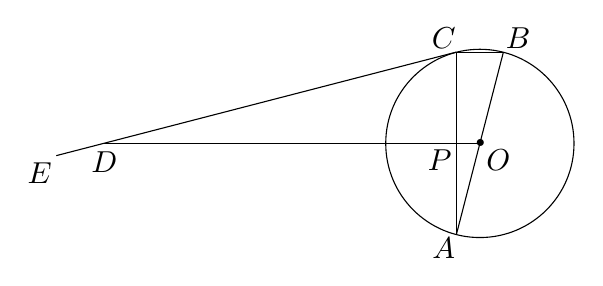
\begin{tikzpicture}[x=1pt, y=1pt,
    every node/.style={inner sep=0pt, font=\fontsize{10.5pt}{12.6pt}\selectfont}]

  % ---- 圆：m + 4c + h（源内容流 path 41，lw 0.398） ----
  % 源真页坐标：m (695.7345,608.2880)
  %   c (695.7345,627.0750) (680.5055,642.3040) (661.7185,642.3040)
  %   c (642.9305,642.3040) (627.7015,627.0750) (627.7015,608.2880)
  %   c (627.7015,589.5010) (642.9305,574.2720) (661.7185,574.2720)
  %   c (680.5055,574.2720) (695.7345,589.5010) (695.7345,608.2880)  h
  \draw[line width=0.398pt]
    (68.0330,34.0160)
    .. controls (68.0330,52.8030) and (52.8040,68.0320) .. (34.0170,68.0320)
    .. controls (15.2290,68.0320) and (0.0000,52.8030) .. (0.0000,34.0160)
    .. controls (0.0000,15.2290) and (15.2290,0.0000) .. (34.0170,0.0000)
    .. controls (52.8040,0.0000) and (68.0330,15.2290) .. (68.0330,34.0160)
    -- cycle;

  % ---- AC（源 path 42，lw 0.398）：A(653.2134,575.2900) → C(653.2134,641.2860) ----
  \draw[line width=0.398pt] (25.5119,1.0180) -- (25.5119,67.0140);

  % ---- BC（源 path 43，lw 0.398）：B(670.2226,641.2860) → C(653.2136,641.2860) ----
  \draw[line width=0.398pt] (42.5211,67.0140) -- (25.5121,67.0140);

  % ---- AB（源 path 44，lw 0.398）：A(653.2134,575.2900) → B(670.2224,641.2860) ----
  \draw[line width=0.398pt] (25.5119,1.0180) -- (42.5209,67.0140);

  % ---- DO（源 path 45，lw 0.398）：O(661.7180,608.2880) → D(525.6440,608.2880) ----
  \draw[line width=0.398pt] (34.0165,34.0160) -- (-102.0575,34.0160);

  % ---- EC 切线（源 path 46，lw 0.398）：C(653.2134,641.2860) → E(508.6344,603.8660) ----
  \draw[line width=0.398pt] (25.5119,67.0140) -- (-119.0671,29.5940);

  % ---- 标签：源文本 Tm 原点（基线左端），CMMI10 10.5pt ----
  \node[anchor=base west] at (16.6435,-7.5010)  {$A$};   % 源 (644.3450,566.7710)
  \node[anchor=base west] at (43.2065,68.3580)  {$B$};   % 源 (670.9080,642.6300)
  \node[anchor=base west] at (16.4485,68.3580)  {$C$};   % 源 (644.1500,642.6300)
  \node[anchor=base west] at (-106.5505,23.4550) {$D$};  % 源 (521.1510,597.7270)
  \node[anchor=base west] at (-129.5855,19.6660) {$E$};  % 源 (498.1160,593.9380)
  \node[anchor=base west] at (36.2065,24.0880)  {$O$};   % 源 (663.9080,598.3600)
  \node[anchor=base west] at (15.0715,24.0880)  {$P$};   % 源 (642.7730,598.3600)
  % 圆心点：源 CMSY10 0x0F（`\bullet`），Tm 为 0.6 缩放（CMSY10 10.5pt × 0.6），
  % 基线原点 (660.1428,606.8878) → 本地 (32.4413,32.6158)。
  \node[anchor=base west, scale=0.6] at (32.4413,32.6158) {$\bullet$};

\end{tikzpicture}
%
% 【自验结果】
%   探针：latexmk -pdfxe，0 error / 0 Overfull / 0 Underfull / 0 Missing character；
%         页面 200.38 × 82.72 pt（standalone border=0）。
%   tex 反算：6 条路径 + 8 个标签全部匹配，最大残差 0.000000 pt（阈值 0.05）。
%   600dpi 墨迹：整体墨迹包围盒最大边差 0.209 pt；几何包围盒 0.123 pt；
%         标签中心最大 0.295 pt（D）。（尺度归一，已扣除探针
%         0.996276 = 72/72.27 的 TeX pt / PDF bp 均匀因子）
%         按页面 bp 直接比较（物理）最大 0.679 pt，全部来自该 0.37% 均匀缩放。
%   灵敏度：端点 E +0.15pt → tex 检查器报 0.1500、600dpi 几何包围盒报 0.2409；
%         标签 C +0.15pt → tex 检查器报 0.1500、600dpi 标签中心报 0.0868。均能报出。
\end{center}
\nopagebreak[4]
\Needspace{4\baselineskip}
\textbf{解析}

\Needspace{5\baselineskip}
以 \(O\) 为原点、\(AB\) 所在直线为 \(x\) 轴，取 \(B(2,0)\)、\(A(-2,0)\)（半径 \(R=2\)）。设 \(C(x_0,y_0)\)，由 \(OC=2\)、\(BC=1\)：
\nopagebreak[4]
\[
x_0^2+y_0^2=4,\qquad (x_0-2)^2+y_0^2=1.
\]
\Needspace{5\baselineskip}
相减得 \(-4x_0+4=-3\)，即 \(x_0=\dfrac74\)，从而
\nopagebreak[4]
\[
y_0^2=4-\frac{49}{16}=\frac{15}{16},\qquad y_0=\frac{\sqrt{15}}{4}
\]
（另一侧对称，结果相同）。

\Needspace{5\baselineskip}
过 \(C\) 的切线方程为 \(\dfrac74x+\dfrac{\sqrt{15}}4y=4\)，即
\nopagebreak[4]
\[
7x+\sqrt{15}\,y=16.
\]
\Needspace{5\baselineskip}
直线 \(BC\) 的方向为 \(C-B=\left(-\dfrac14,\dfrac{\sqrt{15}}4\right)\)，故过 \(O\) 且平行于 \(BC\) 的直线为
\nopagebreak[4]
\[
y=-\sqrt{15}\,x.
\]
\Needspace{5\baselineskip}
联立：
\nopagebreak[4]
\[
7x+\sqrt{15}\cdot(-\sqrt{15}x)=16
\ \Longrightarrow\ 7x-15x=16
\ \Longrightarrow\ x=-2,
\]
\Needspace{5\baselineskip}
从而 \(y=2\sqrt{15}\)。故 \(D(-2,2\sqrt{15})\)，
\nopagebreak[4]
\[
OD=\sqrt{(-2)^2+(2\sqrt{15})^2}=\sqrt{4+60}=8.
\]

\Needspace{5\baselineskip}
（验证（几何法）：\(AB\) 为直径，故 \(P\) 为 \(AC\) 中点，\(OP\parallel BC\)；切线 \(CD\perp OC\)。在 \(\mathrm{Rt}\triangle OCD\) 中 \(\angle COD=\angle OCB\)。等腰 \(\triangle OBC\)（\(OB=OC=2\)，\(BC=1\)）中
\nopagebreak[4]
\[
\cos\angle OCB=\frac{OC^2+BC^2-OB^2}{2\cdot OC\cdot BC}=\frac{4+1-4}{4}=\frac14,
\]
故 \(OD=\dfrac{OC}{\cos\angle COD}=\dfrac{2}{1/4}=8\)，与坐标法一致。）

\gkanswer{答案：\(8\)}

\end{answer}
\begin{answer}
\gksolhead{16}{平面向量}

\textbf{题目}：

在平面直角坐标系 \(xOy\) 中，已知向量 \(\boldsymbol{m}=\left(\dfrac{\sqrt{2}}{2},-\dfrac{\sqrt{2}}{2}\right)\)，\(\boldsymbol{n}=(\sin x,\cos x)\)，\(x\in\left(0,\dfrac{\pi}{2}\right)\)。

（1） 若 \(\boldsymbol{m}\perp\boldsymbol{n}\)，求 \(\tan x\) 的值；

（2） 若 \(\boldsymbol{m}\) 与 \(\boldsymbol{n}\) 的夹角为 \(\dfrac{\pi}{3}\)，求 \(x\) 的值。

\Needspace{4\baselineskip}
\textbf{解析}

\gksubpart{(1)}

\Needspace{5\baselineskip}
由 \(\boldsymbol{m}\perp\boldsymbol{n}\) 得
\nopagebreak[4]
\[
\boldsymbol{m}\cdot\boldsymbol{n}=\frac{\sqrt2}{2}\sin x-\frac{\sqrt2}{2}\cos x=0,
\]
\Needspace{5\baselineskip}
即 \(\sin x=\cos x\)。因 \(x\in\left(0,\dfrac{\pi}{2}\right)\)，\(\cos x\ne0\)（若 \(\cos x=0\)，则 \(\sin x=1\)，不满足 \(\sin x=\cos x\)），故
\nopagebreak[4]
\[
\tan x=1,
\]
此时 \(x=\dfrac{\pi}{4}\)。

（验证：\(x=\dfrac{\pi}{4}\) 时 \(\boldsymbol{m}\cdot\boldsymbol{n}=\dfrac{\sqrt2}{2}\cdot\dfrac{\sqrt2}{2}-\dfrac{\sqrt2}{2}\cdot\dfrac{\sqrt2}{2}=0\)。）

\gksubpart{(2)}

\Needspace{4\baselineskip}
\textbf{解析}

\nopagebreak[4]
\[
|\boldsymbol{m}|=\sqrt{\frac12+\frac12}=1,\qquad
|\boldsymbol{n}|=\sqrt{\sin^2x+\cos^2x}=1.
\]
\Needspace{5\baselineskip}
夹角为 \(\dfrac{\pi}{3}\)，故
\nopagebreak[4]
\[
\boldsymbol{m}\cdot\boldsymbol{n}=|\boldsymbol{m}||\boldsymbol{n}|\cos\frac{\pi}{3}=\frac12.
\]
\Needspace{5\baselineskip}
即
\nopagebreak[4]
\[
\frac{\sqrt2}{2}(\sin x-\cos x)=\frac12
\ \Longrightarrow\ \sin x-\cos x=\frac{\sqrt2}{2}.
\]
\Needspace{5\baselineskip}
由辅助角公式，
\nopagebreak[4]
\[
\sqrt2\sin\left(x-\frac{\pi}{4}\right)=\frac{\sqrt2}{2}
\ \Longrightarrow\ \sin\left(x-\frac{\pi}{4}\right)=\frac12.
\]
\Needspace{5\baselineskip}
由 \(x\in\left(0,\dfrac{\pi}{2}\right)\) 得 \(x-\dfrac{\pi}{4}\in\left(-\dfrac{\pi}{4},\dfrac{\pi}{4}\right)\)，故
\nopagebreak[4]
\[
x-\frac{\pi}{4}=\frac{\pi}{6},\qquad x=\frac{5\pi}{12}.
\]

（验证：\(\sin\dfrac{5\pi}{12}=\dfrac{\sqrt6+\sqrt2}{4}\)，\(\cos\dfrac{5\pi}{12}=\dfrac{\sqrt6-\sqrt2}{4}\)，差为 \(\dfrac{\sqrt2}{2}\)，故 \(\boldsymbol{m}\cdot\boldsymbol{n}=\dfrac12\)，夹角为 \(\dfrac{\pi}{3}\)。）

\gkanswer{答案（1）：\(\tan x=1\)（此时 \(x=\dfrac{\pi}{4}\)）。}

\gkanswer{答案（2）：\(x=\dfrac{5\pi}{12}\)。}

\end{answer}
\begin{answer}
\gksolhead{17}{统计}

\textbf{题目}：

某工厂 36 名工人的年龄数据如下表。

\begin{center}
\begingroup\setlength{\tabcolsep}{4pt}
\begin{tabular}{cccccccc}
\toprule
工人编号 & 年龄 & 工人编号 & 年龄 & 工人编号 & 年龄 & 工人编号 & 年龄 \\
\midrule
1 & 40 & 10 & 36 & 19 & 27 & 28 & 34 \\
2 & 44 & 11 & 31 & 20 & 43 & 29 & 39 \\
3 & 40 & 12 & 38 & 21 & 41 & 30 & 43 \\
4 & 41 & 13 & 39 & 22 & 37 & 31 & 38 \\
5 & 33 & 14 & 43 & 23 & 34 & 32 & 42 \\
6 & 40 & 15 & 45 & 24 & 42 & 33 & 53 \\
7 & 45 & 16 & 39 & 25 & 37 & 34 & 37 \\
8 & 42 & 17 & 38 & 26 & 44 & 35 & 49 \\
9 & 43 & 18 & 36 & 27 & 42 & 36 & 39 \\
\bottomrule
\end{tabular}
\endgroup
\end{center}

（1） 用系统抽样法从 36 名工人中抽取容量为 9 的样本，且在第一分段里用随机抽样法抽到的年龄数据为 44，列出样本的年龄数据；

（2） 计算（1）中样本的均值 \(\bar{x}\) 和方差 \(s^2\)；

（3） 36 名工人中年龄在 \(\bar{x}-s\) 与 \(\bar{x}+s\) 之间有多少人？所占的百分比是多少（精确到 \(0.01\%\)）？

\Needspace{4\baselineskip}
\textbf{解析}

\gksubpart{(1)}

\Needspace{5\baselineskip}
\(36\) 人分 \(9\) 段，每段 \(4\) 人。第一段（\(1\sim4\) 号）抽到年龄 \(44\)，即 \(2\) 号工人，故各段均取第 \(2\) 位，编号为
\nopagebreak[4]
\[
2,6,10,14,18,22,26,30,34.
\]
\Needspace{5\baselineskip}
查表得样本年龄数据为
\nopagebreak[4]
\[
44,40,36,43,36,37,44,43,37.
\]

（验证：相邻编号差均为 \(4\)，落在 \(1\sim36\) 内且每段恰取一个。）

\gksubpart{(2)}

\Needspace{4\baselineskip}
\textbf{解析}

\nopagebreak[4]
\[
\bar{x}=\frac{44+40+36+43+36+37+44+43+37}{9}=\frac{360}{9}=40.
\]
\Needspace{5\baselineskip}
各数据与均值的偏差为 \(4,0,-4,3,-4,-3,4,3,-3\)，平方和为
\nopagebreak[4]
\[
16+0+16+9+16+9+16+9+9=100,
\]
\Needspace{5\baselineskip}
故
\nopagebreak[4]
\[
s^2=\frac{100}{9}.
\]

（验证：偏差代数和 \(4+0-4+3-4-3+4+3-3=0\)，均值计算无误；平方和逐项复核为 \(100\)。）

\gksubpart{(3)}

\Needspace{4\baselineskip}
\textbf{解析}

\nopagebreak[4]
\[
\bar{x}-s=40-\frac{10}{3}=\frac{110}{3}\approx36.67,\qquad
\bar{x}+s=40+\frac{10}{3}=\frac{130}{3}\approx43.33.
\]
\Needspace{5\baselineskip}
统计 \(36\) 人中年龄严格介于 \(\dfrac{110}{3}\) 与 \(\dfrac{130}{3}\) 之间者，即年龄为 \(37,38,39,40,41,42,43\) 的工人：
\nopagebreak[4]
\[
3+3+4+3+2+4+4=23\ \text{人}.
\]
\Needspace{5\baselineskip}
故所占百分比为
\nopagebreak[4]
\[
\frac{23}{36}\times100\%=63.888\ldots\%\approx63.89\%.
\]

（验证：区间外的 \(13\) 人年龄为 \(44,33,45,36,31,45,36,27,34,44,34,53,49\)，\(13+23=36\)，总人数吻合。）

\gkanswer{答案（1）：样本年龄 \(44,40,36,43,36,37,44,43,37\)（编号 \(2,6,10,14,18,22,26,30,34\)）。}

\gkanswer{答案（2）：\(\bar{x}=40\)，\(s^2=\dfrac{100}{9}\)。}

\gkanswer{答案（3）：\(23\) 人，占 \(63.89\%\)。}

\end{answer}
\begin{answer}
\gksolhead{18}{立体几何}

\textbf{题目}：

如图，三角形 \(PDC\) 所在的平面与长方形 \(ABCD\) 所在的平面垂直，\(PD=PC=4\)，\(AB=6\)，\(BC=3\)。点 \(E\) 是 \(CD\) 边的中点，点 \(F\)，\(G\) 分别在线段 \(AB\)，\(BC\) 上，且 \(AF=2FB\)，\(CG=2GB\)。

（1） 证明：\(PE\perp FG\)；

（2） 求二面角 \(P-AD-C\) 的正切值；

（3） 求直线 \(PA\) 与直线 \(FG\) 所成角的余弦值。
\nopagebreak[4]
\begin{center}% f2015gdl_q18_solid.tex — 2015 年高考数学·广东卷·理科 第 18 题（四棱锥 P-ABCD 立体图）
%
% 【来源】`.work/phase3-b17/source/2015广东理.pdf`（SHA-256
%   1c3faab50a5d1fb2bdba424104c10910341e7362d222e018fb27e631578daa9a），
%   第 2 页（合订本页 948）第 1 栏；内容对象 21。
%
% 【坐标口径】清单坐标为「真页 pt、原点左上、y 向下」。本图取
%   X0 = 202.0221（顶点 A 的 x），Y0 = 284.7441（顶点 A 的 y_top），
%   本地坐标  (x, y) = (x_page − X0, Y0 − y_top)，即本地原点 = 顶点 A，
%   x 向右、y 向上，1 单位 = 1 TeX pt。
%   换算示例：A (202.0221,284.7441) → (0,0)；B (365.2908,284.7441) → (163.2687,0)；
%   C (389.7813,243.9270) → (187.7592,40.8171)；D (226.5127,243.9270) → (24.4906,40.8171)；
%   P (308.1470,171.9323) → (106.1249,112.8118)。
%
% 【与广东文卷 Q18 的关系】本图几何与 `2015_广东卷_文科` Q18 图相同（x 逐点相同），
%   整体在页面上比文卷版下移 10.627pt；理科版新增 E（CD 中点）、F、G 三要素与
%   P–E、G–F 两条线段。文理互证由主会话事后完成，图源照本卷源件独立实测。
%
% 【线宽/虚线】全部棱 line width = 0.3985pt；DC 短段 dash pattern =
%   on 2.98883pt off 2.98883pt，dash phase = 0pt；无填充、无 c 算子（全为 m/l 直线）。
%
% 【照源复刻的存疑项】
%   DC 自 D 起为虚线：虚线路径为「交点 → D」（源 m (240.1184,597.9630)
%   l (226.5127,597.9630) 方向照录），相位 0 起于交点。
%   源未画棱 PB，照录不补。
%   源每条棱路径起点有零长度重复 moveto，按规范不复刻。
%
% 【自验结果】见文件末尾。
%
% 元素计数：11 条路径（9 条实线棱/线段 + DC 实线 + DC 虚线）、8 个标签。
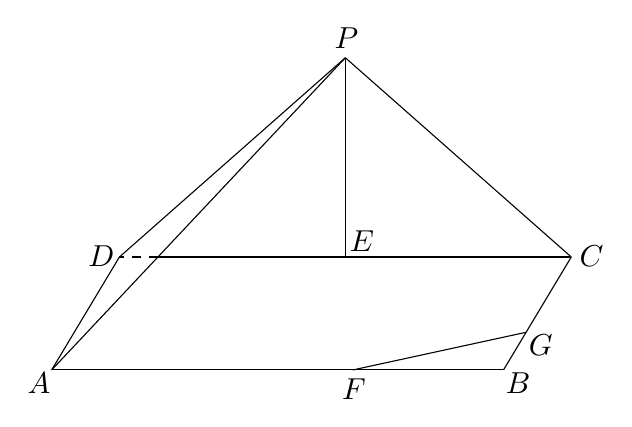
\begin{tikzpicture}[x=1pt, y=1pt,
    every node/.style={inner sep=0pt, font=\fontsize{10.5pt}{12.6pt}\selectfont}]

  % ---- 顶点（本地坐标） ----
  % A (0,0)  B (163.2687,0)  C (187.7592,40.8171)  D (24.4906,40.8171)
  % P (106.1249,112.8118)  E (106.1249,40.8171)  F (108.8458,0)  G (171.4322,13.6057)

  % ---- P–D（源 path 0：m D(226.5127,597.9630) l P(308.1470,669.9577)，本图反向） ----
  \draw[line width=0.3985pt] (106.1249,112.8118) -- (24.4906,40.8171);

  % ---- P–C（源 path 1：m P(308.1470,669.9577) l C(389.7813,597.9630)） ----
  \draw[line width=0.3985pt] (106.1249,112.8118) -- (187.7592,40.8171);

  % ---- A–D（源 path 2：m A(202.0221,557.1459) l D(226.5127,597.9630)） ----
  \draw[line width=0.3985pt] (0.0000,0.0000) -- (24.4906,40.8171);

  % ---- A–B（源 path 3：m B(365.2908,557.1459) l A(202.0221,557.1459)，本图反向） ----
  \draw[line width=0.3985pt] (0.0000,0.0000) -- (163.2687,0.0000);

  % ---- G–F（源 path 4：m G(373.4543,570.7516) l F(310.8679,557.1459)） ----
  \draw[line width=0.3985pt] (171.4322,13.6057) -- (108.8458,0.0000);

  % ---- A–P（源 path 5：m A(202.0221,557.1459) l P(308.1470,669.9577)） ----
  \draw[line width=0.3985pt] (0.0000,0.0000) -- (106.1249,112.8118);

  % ---- B–C（源 path 6：m B(365.2908,557.1459) l C(389.7813,597.9630)） ----
  \draw[line width=0.3985pt] (163.2687,0.0000) -- (187.7592,40.8171);

  % ---- P–E（源 path 7：m P(308.1470,669.9577) l E(308.1470,597.9630)） ----
  \draw[line width=0.3985pt] (106.1249,112.8118) -- (106.1249,40.8171);

  % ---- D–C 实线段（源 path 8：m C(389.7813,597.9630) l (240.1184,597.9630)） ----
  \draw[line width=0.3985pt] (187.7592,40.8171) -- (38.0963,40.8171);

  % ---- D–C 虚线段（源 path 9：m (240.1184,597.9630) l D(226.5127,597.9630)，方向照源） ----
  \draw[line width=0.3985pt, dash pattern=on 2.98883pt off 2.98883pt, dash phase=0pt]
    (38.0963,40.8171) -- (24.4906,40.8171);

  % ---- 标签：源文本 Tm 原点（基线左端），CMMI10 10.5pt ----
  \node[anchor=base west] at (102.0249,116.1981) {$P$};  % 源 (304.0470,673.3440)
  \node[anchor=base west] at (13.0239,37.2291)   {$D$};  % 源 (215.0460,594.3750)
  \node[anchor=base west] at (190.6049,37.2291)  {$C$};  % 源 (392.6270,594.3750)
  \node[anchor=base west] at (-8.8691,-8.5189)   {$A$};  % 源 (193.1530,548.6270)
  \node[anchor=base west] at (163.9539,-8.5189)  {$B$};  % 源 (365.9760,548.6270)
  \node[anchor=base west] at (107.5829,42.8651)  {$E$};  % 源 (309.6050,600.0110)
  \node[anchor=base west] at (104.7409,-10.5619) {$F$};  % 源 (306.7630,546.5840)
  \node[anchor=base west] at (172.2359,5.0871)   {$G$};  % 源 (374.2580,562.2330)

\end{tikzpicture}
%
% 【自验结果】
%   探针：latexmk -pdfxe，0 error / 0 Overfull / 0 Underfull / 0 Missing character；
%         页面 210.45 × 133.43 pt（standalone border=0）。
%   tex 反算：10 条路径 + 8 个标签全部匹配，最大残差 0.000050 pt（阈值 0.05）。
%   600dpi 墨迹：整体墨迹包围盒最大边差 0.325 pt；几何包围盒 0.065 pt；
%         标签中心最大 0.298 pt（C）。（尺度归一，已扣除 0.996277 的
%         TeX pt / PDF bp 均匀因子）
%         按页面 bp 直接比较（物理）最大 0.655 pt，来自该 0.37% 均匀缩放。
%   灵敏度：顶点 C x +0.15pt → tex 检查器报 0.1500、600dpi 几何包围盒报 0.1204；
%         标签 E y +0.15pt → tex 检查器报 0.1500、600dpi 标签中心报 0.0946；
%         G–F 线宽 +0.02pt → 等效宽度 0.9094 → 0.9517 pt（delta +0.0423）。均能报出。
\end{center}
\nopagebreak[4]
\Needspace{4\baselineskip}
\textbf{解析}

\gksubpart{(1)}

因 \(PD=PC\) 且 \(E\) 为 \(CD\) 中点，故 \(PE\perp CD\)。又平面 \(PDC\perp\) 平面 \(ABCD\)，交线为 \(CD\)，\(PE\subset\) 平面 \(PDC\)，故 \(PE\perp\) 平面 \(ABCD\)。

\Needspace{5\baselineskip}
取 \(E\) 为原点，\(DC\) 为 \(x\) 轴，平行于 \(AD\) 的方向为 \(y\) 轴，\(EP\) 为 \(z\) 轴，则
\nopagebreak[4]
\[
E(0,0,0),\quad D(-3,0,0),\quad C(3,0,0),\quad B(3,-3,0),\quad A(-3,-3,0).
\]
\Needspace{5\baselineskip}
由 \(PD=4\)，\(PE=\sqrt{4^2-3^2}=\sqrt7\)，得 \(P(0,0,\sqrt7)\)。又 \(AF=2FB\)，\(AB=6\)，得 \(AF=4\)，\(F(1,-3,0)\)；\(CG=2GB\)，\(BC=3\)，得 \(CG=2\)，\(G(3,-2,0)\)。于是
\nopagebreak[4]
\[
\overrightarrow{PE}=(0,0,-\sqrt7),\qquad \overrightarrow{FG}=(2,1,0),
\]
\nopagebreak[4]
\[
\overrightarrow{PE}\cdot\overrightarrow{FG}=0\cdot2+0\cdot1+(-\sqrt7)\cdot0=0,
\]
故 \(PE\perp FG\)。

（验证：\(PE\) 沿 \(z\) 轴方向，\(FG\) 在 \(z=0\) 平面内且无 \(z\) 分量，点积为 \(0\) 即证。）

\gksubpart{(2)}

\Needspace{4\baselineskip}
\textbf{解析}

\Needspace{5\baselineskip}
平面 \(ABCD\) 的法向量可取 \(\boldsymbol{n}_2=(0,0,1)\)。平面 \(PAD\) 中
\nopagebreak[4]
\[
\overrightarrow{AD}=(0,3,0),\qquad \overrightarrow{AP}=(3,3,\sqrt7),
\]
\Needspace{5\baselineskip}
法向量可取
\nopagebreak[4]
\[
\boldsymbol{n}_1=\overrightarrow{AD}\times\overrightarrow{AP}=(3\sqrt7,0,-9)\parallel(\sqrt7,0,-3).
\]
\Needspace{5\baselineskip}
设二面角为 \(\theta\)，则
\nopagebreak[4]
\[
\cos\theta=\frac{|\boldsymbol{n}_1\cdot\boldsymbol{n}_2|}{|\boldsymbol{n}_1||\boldsymbol{n}_2|}
=\frac{3}{\sqrt{7+9}}=\frac34,
\]
\Needspace{5\baselineskip}
故 \(\sin\theta=\dfrac{\sqrt7}{4}\)，
\nopagebreak[4]
\[
\tan\theta=\frac{\sin\theta}{\cos\theta}=\frac{\sqrt7}{3}.
\]

（验证（几何法）：在垂直于棱 \(AD\) 的截面内，\(E\) 到 \(AD\) 的距离为 \(3\)，\(PE=\sqrt7\)，故 \(\tan\theta=\dfrac{PE}{3}=\dfrac{\sqrt7}{3}\)，一致。）

\gksubpart{(3)}

\Needspace{4\baselineskip}
\textbf{解析}

\nopagebreak[4]
\[
\overrightarrow{PA}=(-3,-3,-\sqrt7),\qquad |\overrightarrow{PA}|=\sqrt{9+9+7}=5;
\]
\nopagebreak[4]
\[
\overrightarrow{FG}=(2,1,0),\qquad |\overrightarrow{FG}|=\sqrt5.
\]
\Needspace{5\baselineskip}
于是
\nopagebreak[4]
\[
\cos\langle PA,FG\rangle
=\frac{|\overrightarrow{PA}\cdot\overrightarrow{FG}|}{|\overrightarrow{PA}||\overrightarrow{FG}|}
=\frac{|(-3)\cdot2+(-3)\cdot1+0|}{5\sqrt5}
=\frac{9}{5\sqrt5}=\frac{9\sqrt5}{25}.
\]

（验证：\(\dfrac{9}{5\sqrt5}\approx0.805<1\)；改用 \(\overrightarrow{AP}=(3,3,\sqrt7)\) 与 \(\overrightarrow{FG}\) 点积为 \(9\)，结果相同。）

\gkanswer{答案（1）：成立（\(PE\perp\) 平面 \(ABCD\)，\(FG\subset\) 平面 \(ABCD\)，故 \(PE\perp FG\)）。}

\gkanswer{答案（2）：\(\dfrac{\sqrt{7}}{3}\)。}

\gkanswer{答案（3）：\(\dfrac{9\sqrt{5}}{25}\)。}

\end{answer}
\begin{answer}
\gksolhead{19}{导数}

\textbf{题目}：

设 \(a>1\)，函数 \(f(x)=(1+x^2)\mathrm{e}^x-a\)。

（1） 求 \(f(x)\) 的单调区间；

（2） 证明：\(f(x)\) 在 \((-\infty,+\infty)\) 上仅有一个零点；

（3） 若曲线 \(y=f(x)\) 在点 \(P\) 处的切线与 \(x\) 轴平行，且在点 \(M(m,n)\) 处的切线与直线 \(OP\) 平行（\(O\) 是坐标原点），证明：\(m\leqslant\sqrt[3]{a-\dfrac{2}{\mathrm{e}}}-1\)。

\Needspace{4\baselineskip}
\textbf{解析}

\gksubpart{(1)}

\nopagebreak[4]
\[
f'(x)=2x\mathrm{e}^x+(1+x^2)\mathrm{e}^x
=\mathrm{e}^x(x^2+2x+1)=\mathrm{e}^x(x+1)^2\geqslant0,
\]
等号仅在 \(x=-1\) 处成立。故 \(f(x)\) 在 \(\mathbf{R}\) 上单调递增，单调递增区间为 \((-\infty,+\infty)\)，无递减区间。

（验证：\(\mathrm{e}^x>0\)，\((x+1)^2\geqslant0\)，导数非负且只在一点为零，不改变严格单调性。）

\gksubpart{(2)}

\Needspace{4\baselineskip}
\textbf{解析}

当 \(x\to-\infty\) 时，\((1+x^2)\mathrm{e}^x\to0\)，故 \(f(x)\to-a<0\)；当 \(x\to+\infty\) 时 \(f(x)\to+\infty\)。由连续性，\(f\) 存在零点。又由 (1)，\(f\) 在 \(\mathbf{R}\) 上严格递增，零点唯一。故 \(f(x)\) 在 \((-\infty,+\infty)\) 上仅有一个零点。

（验证：\(f(0)=1-a<0\)；取 \(x=a>1\)，\(f(a)=(1+a^2)\mathrm{e}^a-a>\mathrm{e}^a-a>0\)，零点位于 \((0,a)\) 内且唯一。）

\gksubpart{(3)}

\Needspace{4\baselineskip}
\textbf{解析}

\Needspace{5\baselineskip}
\(P\) 处切线与 \(x\) 轴平行，等价于 \(f'(x_P)=0\)，即 \(x_P=-1\)。故
\nopagebreak[4]
\[
P\left(-1,\frac{2}{\mathrm{e}}-a\right).
\]
\Needspace{5\baselineskip}
直线 \(OP\) 的斜率为
\nopagebreak[4]
\[
k_{OP}=\frac{\frac{2}{\mathrm{e}}-a-0}{-1-0}=a-\frac{2}{\mathrm{e}}.
\]
\Needspace{5\baselineskip}
\(M(m,n)\) 处切线与 \(OP\) 平行，故
\nopagebreak[4]
\[
f'(m)=\mathrm{e}^m(m+1)^2=a-\frac{2}{\mathrm{e}}.
\]
\Needspace{5\baselineskip}
令 \(h(t)=\mathrm{e}^t-t-1\)，则 \(h'(t)=\mathrm{e}^t-1\)，\(h\) 在 \(t=0\) 处取最小值 \(h(0)=0\)，故对一切实数 \(t\) 有
\nopagebreak[4]
\[
\mathrm{e}^t\geqslant t+1.
\]
\Needspace{5\baselineskip}
取 \(t=m\)，并注意 \((m+1)^2\geqslant0\)，得
\nopagebreak[4]
\[
a-\frac{2}{\mathrm{e}}=\mathrm{e}^m(m+1)^2\geqslant(m+1)^3.
\]
\Needspace{5\baselineskip}
由 \(a>1\) 知 \(a-\dfrac{2}{\mathrm{e}}>0\)，故 \(m+1>0\)。立方根函数单调，于是
\nopagebreak[4]
\[
m+1\leqslant\sqrt[3]{a-\frac{2}{\mathrm{e}}}
\ \Longrightarrow\
m\leqslant\sqrt[3]{a-\frac{2}{\mathrm{e}}}-1.
\]

（验证：\(m=0\) 时 \(\mathrm{e}^0=1=m+1\)，放缩取等；\(a>1\) 保证 \(a-\dfrac{2}{\mathrm{e}}>1-\dfrac{2}{\mathrm{e}}>0\)，立方根有意义；所证不等式方向与 \(\mathrm{e}^m\geqslant m+1\) 一致。）

\gkanswer{答案（1）：单调递增区间为 \((-\infty,+\infty)\)，无递减区间。}

\gkanswer{答案（2）：成立（\(f\) 在 \(\mathbf{R}\) 上严格递增，且 \(x\to-\infty\) 时 \(f(x)\to-a<0\)、\(x\to+\infty\) 时 \(f(x)\to+\infty\)）。}

\gkanswer{答案（3）：成立（由 \(\mathrm{e}^m\geqslant m+1\) 得 \(a-\dfrac{2}{\mathrm{e}}=\mathrm{e}^m(m+1)^2\geqslant(m+1)^3\)，再开立方）。}

\end{answer}
\begin{answer}
\gksolhead{20}{圆与轨迹}

\textbf{题目}：

已知过原点的动直线 \(l\) 与圆 \(C_1\)：\(x^2+y^2-6x+5=0\) 相交于不同的两点 \(A\)，\(B\)。

（1） 求圆 \(C_1\) 的圆心坐标；

（2） 求线段 \(AB\) 的中点 \(M\) 的轨迹 \(C\) 的方程；

（3） 是否存在实数 \(k\)，使得直线 \(L\)：\(y=k(x-4)\) 与曲线 \(C\) 只有一个交点？若存在，求出 \(k\) 的取值范围；若不存在，说明理由。

\Needspace{4\baselineskip}
\textbf{解析}

\gksubpart{(1)}

\nopagebreak[4]
\[
x^2+y^2-6x+5=0
\iff (x-3)^2+y^2=4.
\]
故圆 \(C_1\) 的圆心为 \((3,0)\)，半径为 \(2\)。

（验证：展开 \((x-3)^2+y^2=4\) 即 \(x^2+y^2-6x+5=0\)。）

\gksubpart{(2)}

\Needspace{4\baselineskip}
\textbf{解析}

\Needspace{5\baselineskip}
原点 \(O\) 到圆心 \((3,0)\) 的距离为 \(3>2\)，故 \(O\) 在圆外。设动直线 \(l:y=tx\)（竖直线 \(x=0\) 与圆无交点，不可能是 \(l\)）。\(l\) 与圆有两个不同交点，当且仅当圆心到 \(l\) 的距离小于 \(2\)：
\nopagebreak[4]
\[
\frac{3|t|}{\sqrt{1+t^2}}<2
\iff 5t^2<4
\iff |t|<\frac{2}{\sqrt5}.
\]
\Needspace{5\baselineskip}
设 \(A(x_1,y_1)\)，\(B(x_2,y_2)\)，代入圆方程得
\nopagebreak[4]
\[
(1+t^2)x^2-6x+5=0,
\]
\Needspace{5\baselineskip}
故中点 \(M(x,y)\) 满足
\nopagebreak[4]
\[
x=\frac{x_1+x_2}{2}=\frac{3}{1+t^2},\qquad
y=tx=\frac{3t}{1+t^2}.
\]
\Needspace{5\baselineskip}
消去 \(t\)：由 \(y=tx\) 得
\nopagebreak[4]
\[
x^2+y^2=x^2(1+t^2)=3x,
\]
\Needspace{5\baselineskip}
即
\nopagebreak[4]
\[
x^2+y^2-3x=0
\qquad\left(\text{即 }\left(x-\frac32\right)^2+y^2=\frac94\right).
\]
\Needspace{5\baselineskip}
由 \(|t|<\dfrac{2}{\sqrt5}\) 得 \(1+t^2<\dfrac95\)，故 \(x=\dfrac{3}{1+t^2}>\dfrac53\)；又 \(|t|\geqslant0\) 给出 \(x\leqslant3\)（\(t=0\) 时 \(x=3\)）。故轨迹为
\nopagebreak[4]
\[
C:\ x^2+y^2-3x=0,\qquad \frac53<x\leqslant3.
\]

（验证：端点 \(\left(\dfrac53,\pm\dfrac{2\sqrt5}{3}\right)\) 对应 \(l\) 与圆相切，只有一个交点，不在轨迹上；\((3,0)\) 对应 \(t=0\)，在轨迹上。）

\gksubpart{(3)}

\Needspace{4\baselineskip}
\textbf{解析}

\Needspace{5\baselineskip}
将 \(L:y=k(x-4)\) 代入 \(C\) 的圆方程：
\nopagebreak[4]
\[
x^2+k^2(x-4)^2-3x=0
\ \Longrightarrow\
(1+k^2)x^2-(8k^2+3)x+16k^2=0.
\]
\Needspace{5\baselineskip}
判别式
\nopagebreak[4]
\[
\Delta=(8k^2+3)^2-4(1+k^2)\cdot16k^2=9-16k^2.
\]

① 当 \(|k|>\dfrac34\) 时，\(\Delta<0\)，\(L\) 与整圆无交点，交点数为 \(0\)。

\Needspace{5\baselineskip}
② 当 \(|k|=\dfrac34\) 时，相切，切点横坐标
\nopagebreak[4]
\[
x=\frac{8k^2+3}{2(1+k^2)}=\frac{12}{5},
\]
因 \(\dfrac53<\dfrac{12}{5}\leqslant3\)，切点在轨迹 \(C\) 上，恰有 \(1\) 个交点。

\Needspace{5\baselineskip}
③ 当 \(|k|<\dfrac34\) 时，\(L\) 与整圆有两个交点。设
\nopagebreak[4]
\[
g(x)=(1+k^2)x^2-(8k^2+3)x+16k^2,
\]
\Needspace{5\baselineskip}
则
\nopagebreak[4]
\[
g\left(\frac53\right)=\frac{49k^2-20}{9}.
\]
\begin{itemize}
\item 当 \(|k|<\dfrac{2\sqrt5}{7}\) 时，\(g\left(\dfrac53\right)<0\)，即 \(\dfrac53\) 严格介于两根之间，两根中恰有一根大于 \(\dfrac53\)，故与 \(C\) 恰有 \(1\) 个交点；
\item 当 \(|k|=\dfrac{2\sqrt5}{7}\) 时，一根为 \(x=\dfrac53\)（端点，不在 \(C\) 上），另一根为 \(x=\dfrac{64}{23}>\dfrac53\)，故与 \(C\) 恰有 \(1\) 个交点；
\item 当 \(\dfrac{2\sqrt5}{7}<|k|<\dfrac34\) 时，\(g\left(\dfrac53\right)>0\)，且抛物线顶点横坐标 \(\dfrac{8k^2+3}{2(1+k^2)}>\dfrac53\)，故两根均大于 \(\dfrac53\) 且不超过 \(3\)，与 \(C\) 有 \(2\) 个交点。
\end{itemize}

\Needspace{5\baselineskip}
综上，恰有 \(1\) 个交点的 \(k\) 为
\nopagebreak[4]
\[
k\in\left[-\frac{2\sqrt5}{7},\frac{2\sqrt5}{7}\right]\cup\left\{-\frac34,\frac34\right\}.
\]

（验证：\(k=0\) 时 \(L:y=0\) 与整圆交于 \(x=0,3\)，只有 \((3,0)\) 在 \(C\) 上，\(1\) 个交点；\(k=\dfrac34\) 时切点 \(x=\dfrac{12}{5}\) 在 \(C\) 上，\(1\) 个交点；数值扫描确认区间边界与 \(\{ \pm 3/4\}\) 处均为 \(1\) 个交点。）

\gkanswer{答案（1）：圆心 \(C_1(3,0)\)。}

\gkanswer{答案（2）：轨迹 \(C\)：\(x^2+y^2-3x=0\)，且 \(\dfrac{5}{3}<x\leqslant3\)。}

\gkanswer{答案（3）：存在，\(k\in\left[-\dfrac{2\sqrt{5}}{7},\dfrac{2\sqrt{5}}{7}\right]\cup\left\{-\dfrac{3}{4},\dfrac{3}{4}\right\}\)。}

\end{answer}
\begin{answer}
\gksolhead{21}{数列与不等式}

\textbf{题目}：

数列 \(\{a_n\}\) 满足 \(a_1+2a_2+\cdots+na_n=4-\dfrac{n+2}{2^{n-1}}\)，\(n\in\mathbf{N}^*\)。

（1） 求 \(a_3\) 的值；

（2） 求数列 \(\{a_n\}\) 的前 \(n\) 项和 \(T_n\)；

（3） 令 \(b_1=a_1\)，\(b_n=\dfrac{T_{n-1}}{n}+\left(1+\dfrac{1}{2}+\dfrac{1}{3}+\cdots+\dfrac{1}{n}\right)a_n\)（\(n\geqslant2\)），证明：数列 \(\{b_n\}\) 的前 \(n\) 项和 \(S_n\) 满足 \(S_n<2+2\ln n\)。

\Needspace{4\baselineskip}
\textbf{解析}

\gksubpart{(1)}

\Needspace{5\baselineskip}
记 \(S_n'=\sum_{k=1}^{n}ka_k=4-\dfrac{n+2}{2^{n-1}}\)。\(n=2\) 时
\nopagebreak[4]
\[
a_1+2a_2=4-\frac42=2;
\]
\Needspace{5\baselineskip}
\(n=3\) 时
\nopagebreak[4]
\[
a_1+2a_2+3a_3=4-\frac54=\frac{11}{4}.
\]
\Needspace{5\baselineskip}
相减得
\nopagebreak[4]
\[
3a_3=\frac{11}{4}-2=\frac34
\ \Longrightarrow\ a_3=\frac14.
\]

（验证：\(n=1\) 得 \(a_1=1\)，\(n=2\) 得 \(2a_2=1\)，\(a_2=\dfrac12\)，与 \(a_3=\dfrac14\) 构成 \(\dfrac1{2^{n-1}}\)。）

\gksubpart{(2)}

\Needspace{4\baselineskip}
\textbf{解析}

\Needspace{5\baselineskip}
\(n\geqslant2\) 时，
\nopagebreak[4]
\[
na_n=S_n'-S_{n-1}'
=\left[4-\frac{n+2}{2^{n-1}}\right]-\left[4-\frac{n+1}{2^{n-2}}\right]
=\frac{2(n+1)-(n+2)}{2^{n-1}}=\frac{n}{2^{n-1}},
\]
\Needspace{5\baselineskip}
故 \(a_n=\dfrac1{2^{n-1}}\)。\(n=1\) 时 \(a_1=4-\dfrac31=1=\dfrac1{2^0}\)，故对一切 \(n\in\mathbf{N}^*\) 有 \(a_n=2^{1-n}\)。于是
\nopagebreak[4]
\[
T_n=\sum_{k=1}^{n}2^{1-k}
=\frac{1-\left(\frac12\right)^n}{1-\frac12}
=2\left(1-2^{-n}\right)=2-2^{1-n}.
\]

（验证：\(T_1=1\)，\(T_2=1+\dfrac12=\dfrac32=2-\dfrac12\)，\(T_3=\dfrac74=2-\dfrac14\)，均符合。）

\gksubpart{(3)}

\Needspace{4\baselineskip}
\textbf{解析}

\Needspace{5\baselineskip}
记 \(H_n=1+\dfrac12+\cdots+\dfrac1n\)（\(H_1=1\)）。由 (2)，\(T_{n-1}=2-2^{2-n}\)，\(a_n=2^{1-n}\)，故对 \(n\geqslant2\)，
\nopagebreak[4]
\[
b_n=\frac{T_{n-1}}{n}+H_na_n
=\frac{2-2^{2-n}}{n}+\frac{H_n}{2^{n-1}}
=\frac2n+e_n,
\]
\Needspace{5\baselineskip}
其中
\nopagebreak[4]
\[
e_n=\frac{H_n}{2^{n-1}}-\frac{2^{2-n}}{n}.
\]
\Needspace{5\baselineskip}
令
\nopagebreak[4]
\[
g_n=\frac{H_n-\frac1n}{2^{n-2}}.
\]
\Needspace{5\baselineskip}
注意到 \(H_{n+1}-\dfrac1{n+1}=H_n\)，故
\nopagebreak[4]
\[
g_{n+1}=\frac{H_{n+1}-\frac1{n+1}}{2^{n-1}}=\frac{H_n}{2^{n-1}},
\]
\Needspace{5\baselineskip}
从而
\nopagebreak[4]
\[
g_n-g_{n+1}
=\frac{H_n-\frac1n}{2^{n-2}}-\frac{H_n}{2^{n-1}}
=\frac{2H_n-\frac2n-H_n}{2^{n-1}}
=\frac{H_n}{2^{n-1}}-\frac{2^{2-n}}{n}=e_n.
\]
\Needspace{5\baselineskip}
于是
\nopagebreak[4]
\[
\sum_{k=2}^{n}e_k=g_2-g_{n+1}=1-\frac{H_n}{2^{n-1}}
\qquad\left(g_2=\frac{H_2-\frac12}{2^0}=1\right).
\]
\Needspace{5\baselineskip}
所以
\nopagebreak[4]
\[
S_n=b_1+\sum_{k=2}^{n}b_k
=1+\sum_{k=2}^{n}\left(\frac2k+e_k\right)
=1+2(H_n-1)+1-\frac{H_n}{2^{n-1}}
=H_n\left(2-2^{1-n}\right).
\]
\Needspace{5\baselineskip}
因 \(2-2^{1-n}<2\)，得 \(S_n<2H_n\)。又对 \(n\geqslant2\)，
\nopagebreak[4]
\[
\frac1k<\int_{k-1}^{k}\frac{\mathrm{d}x}{x}\quad(k=2,\dots,n)
\ \Longrightarrow\
H_n=1+\sum_{k=2}^{n}\frac1k<1+\int_1^n\frac{\mathrm{d}x}{x}=1+\ln n.
\]
\Needspace{5\baselineskip}
故当 \(n\geqslant2\) 时
\nopagebreak[4]
\[
S_n<2H_n<2(1+\ln n)=2+2\ln n.
\]
\Needspace{5\baselineskip}
当 \(n=1\) 时 \(S_1=b_1=a_1=1<2=2+2\ln1\)。综上，对一切 \(n\in\mathbf{N}^*\)，
\nopagebreak[4]
\[
S_n<2+2\ln n.
\]

（验证：\(S_1=1\)，\(S_2=\dfrac94=2.25\)，\(S_3=\dfrac{77}{24}\approx3.208\)，分别与 \(H_n(2-2^{1-n})\) 一致，且均小于 \(2+2\ln n\)（\(n=2\) 时为 \(3.386\)，\(n=3\) 时为 \(4.197\)）；\(g_k-g_{k+1}=e_k\) 的恒等式可逐项验证（\(k=2\)：\(1-\dfrac34=\dfrac14=e_2\)）。）

\gkanswer{答案（1）：\(a_3=\dfrac{1}{4}\)。}

\gkanswer{答案（2）：\(T_n=2-2^{1-n}\)。}

\gkanswer{答案（3）：成立（\(S_n=H_n\left(2-2^{1-n}\right)<2H_n<2+2\ln n\)）。}

\end{answer}